\begin{figure}[H]
    \begin{subfigure}[t]{.45\textwidth}
        \caption{}
        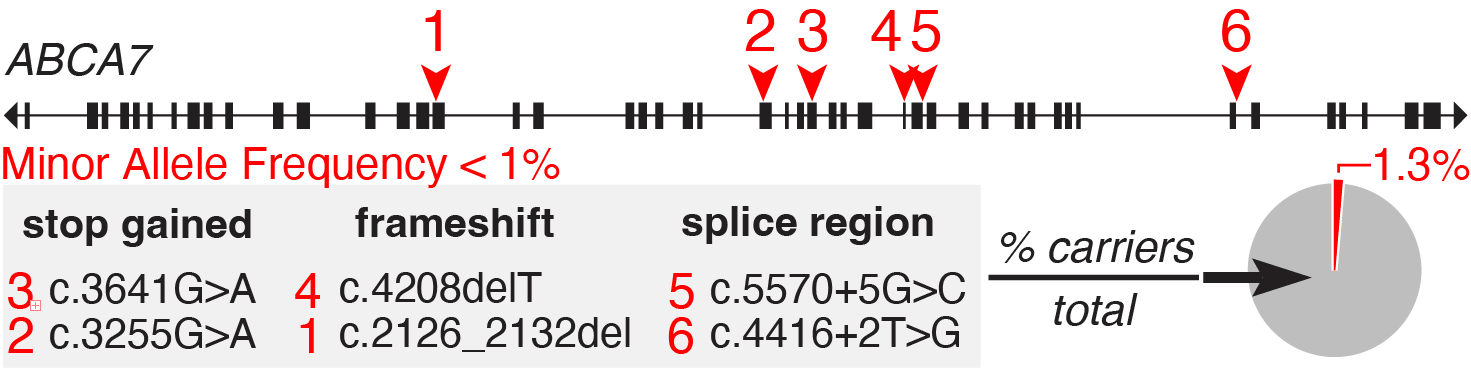
\includegraphics[width=\textwidth]{./main_plots/abca7_variants_cartoon.png}        
    \end{subfigure}
    \begin{subfigure}[t]{.55\textwidth}
        \caption{}
        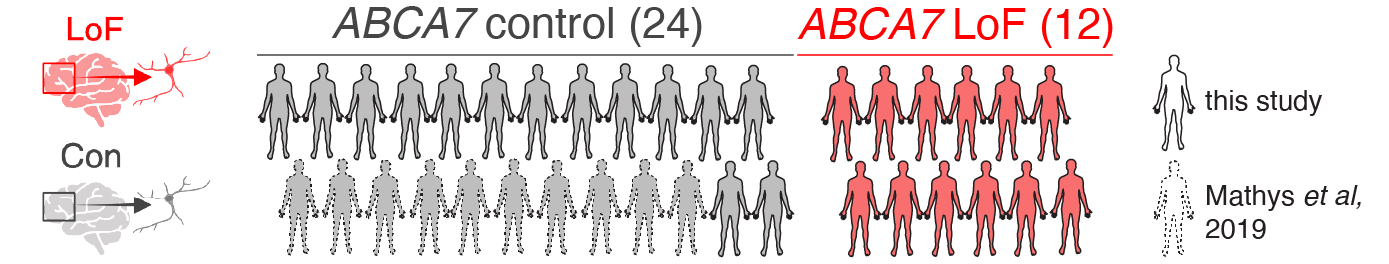
\includegraphics[width=\textwidth]{./main_plots/cohort_cartoon.png}        
    \end{subfigure}
    \\[-1ex] 
    \begin{subfigure}[t]{.5\textwidth}
        \begin{subfigure}[t]{\textwidth}
            \caption{}
            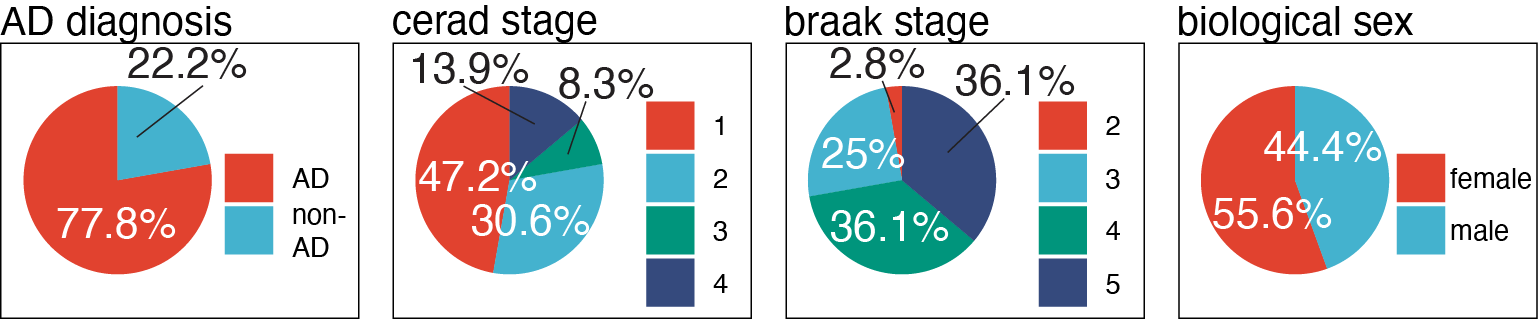
\includegraphics[width=\textwidth]{./main_plots/pie_charts.png}        
        \end{subfigure}
        \begin{subfigure}[t]{.45\textwidth}
            \caption{}
            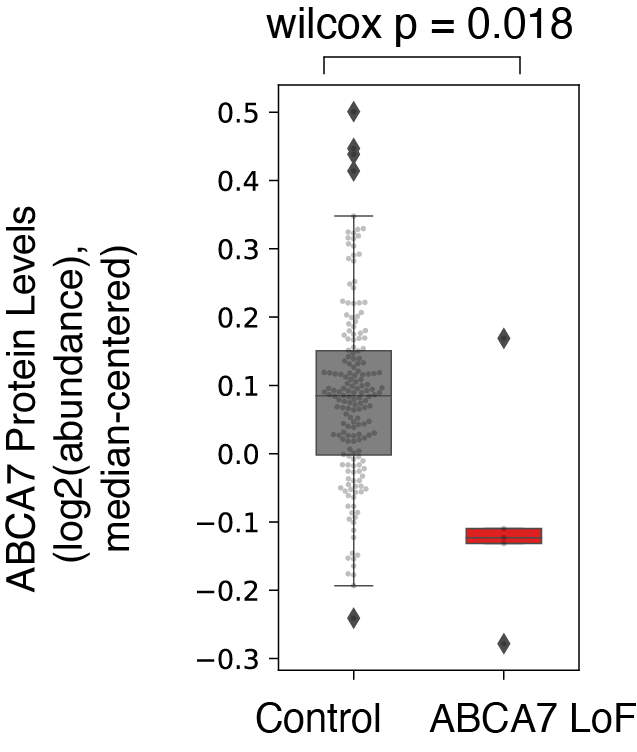
\includegraphics[width=\textwidth]{./main_plots/abca7_protein_levels.png}        
        \end{subfigure}
        \begin{subfigure}[t]{.5\textwidth}
            \caption{}
            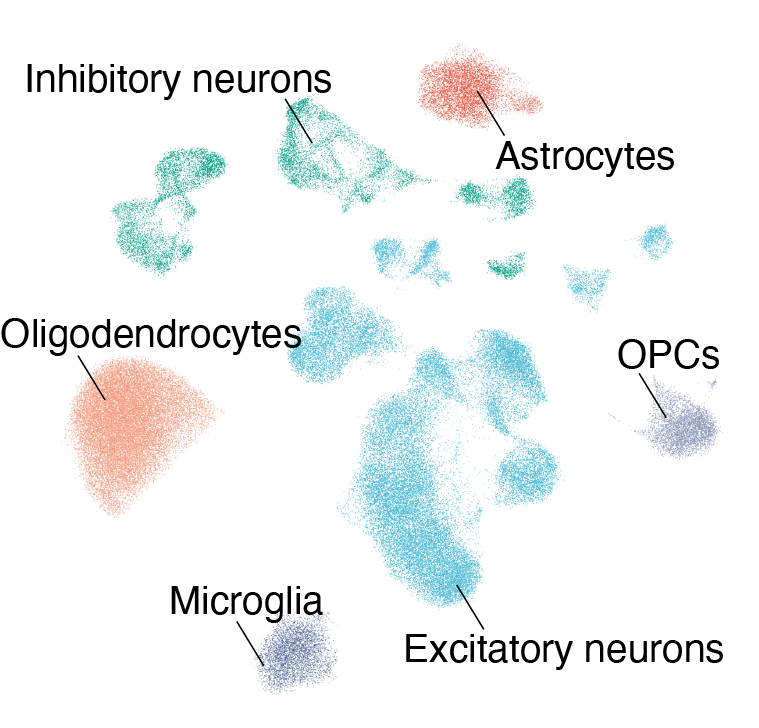
\includegraphics[width=\textwidth]{./main_plots/cell_projection.png}        
        \end{subfigure}
    \\[-3ex] 
    \end{subfigure}
    \begin{subfigure}[t]{0.5\textwidth}
        \caption{}
        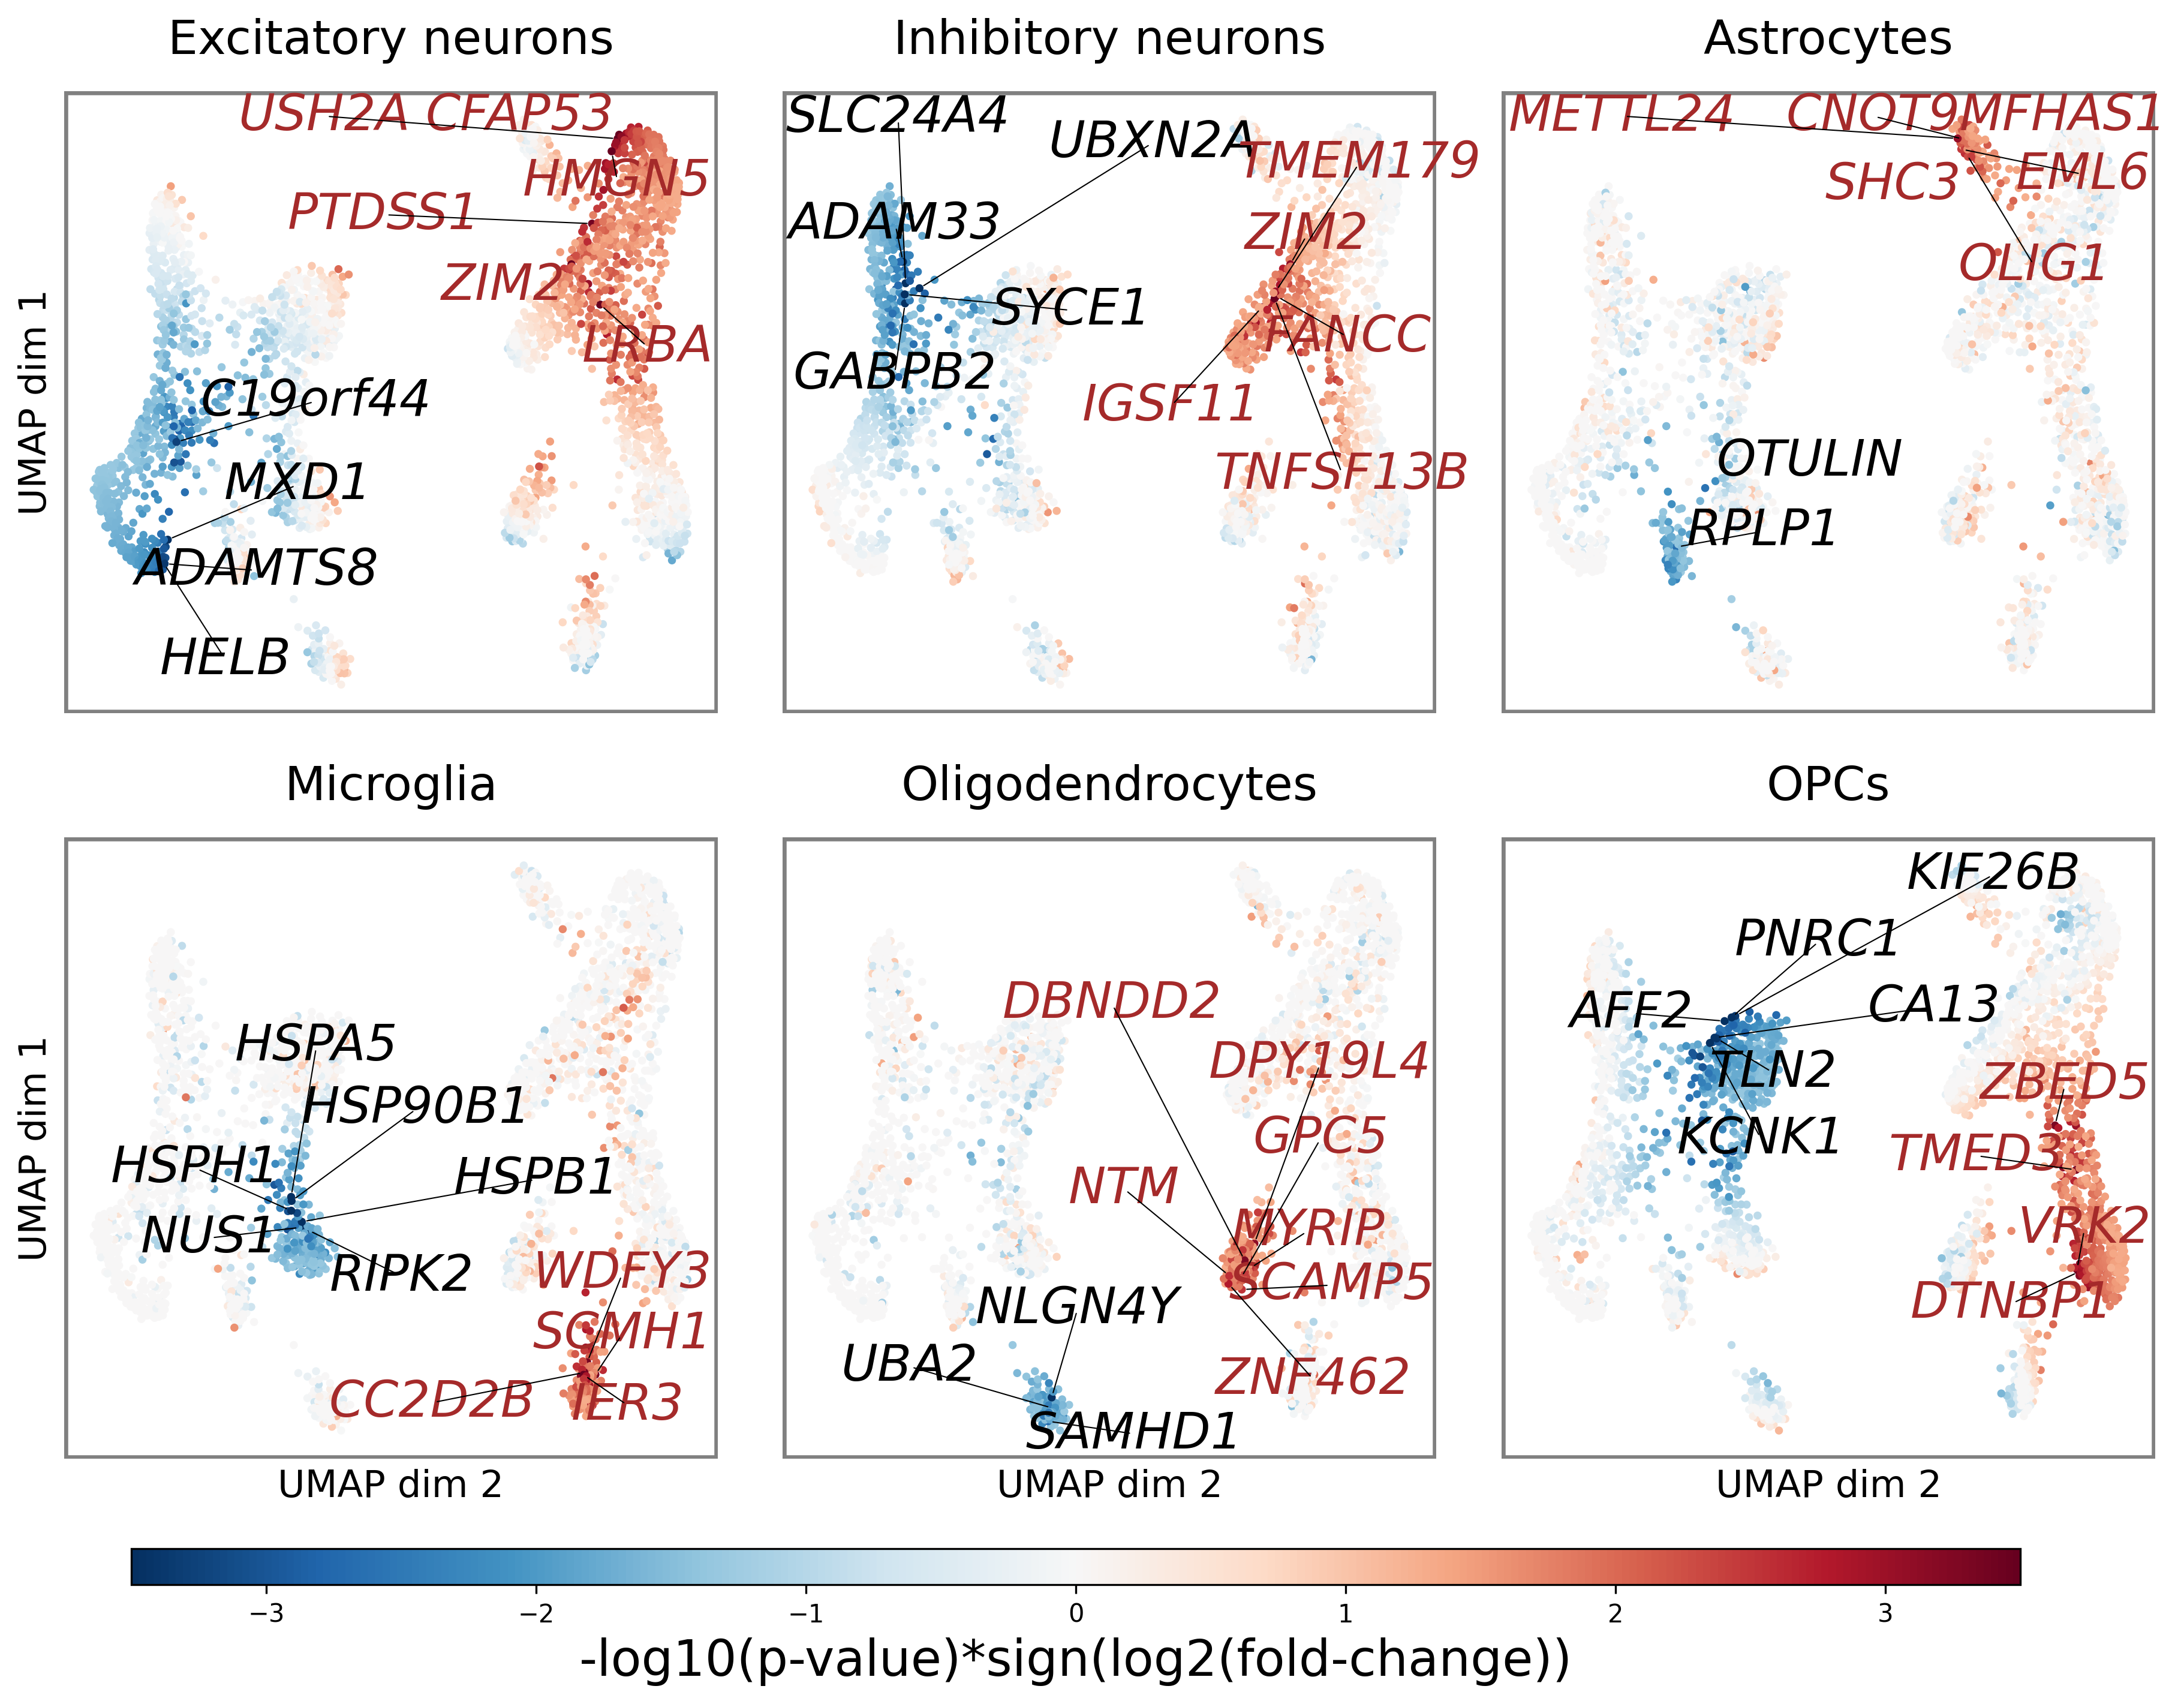
\includegraphics[width=\textwidth]{./main_plots/umap_projection_top_genes.png}        
    \end{subfigure}
    \begin{subfigure}[t]{\textwidth}
        \caption{}
        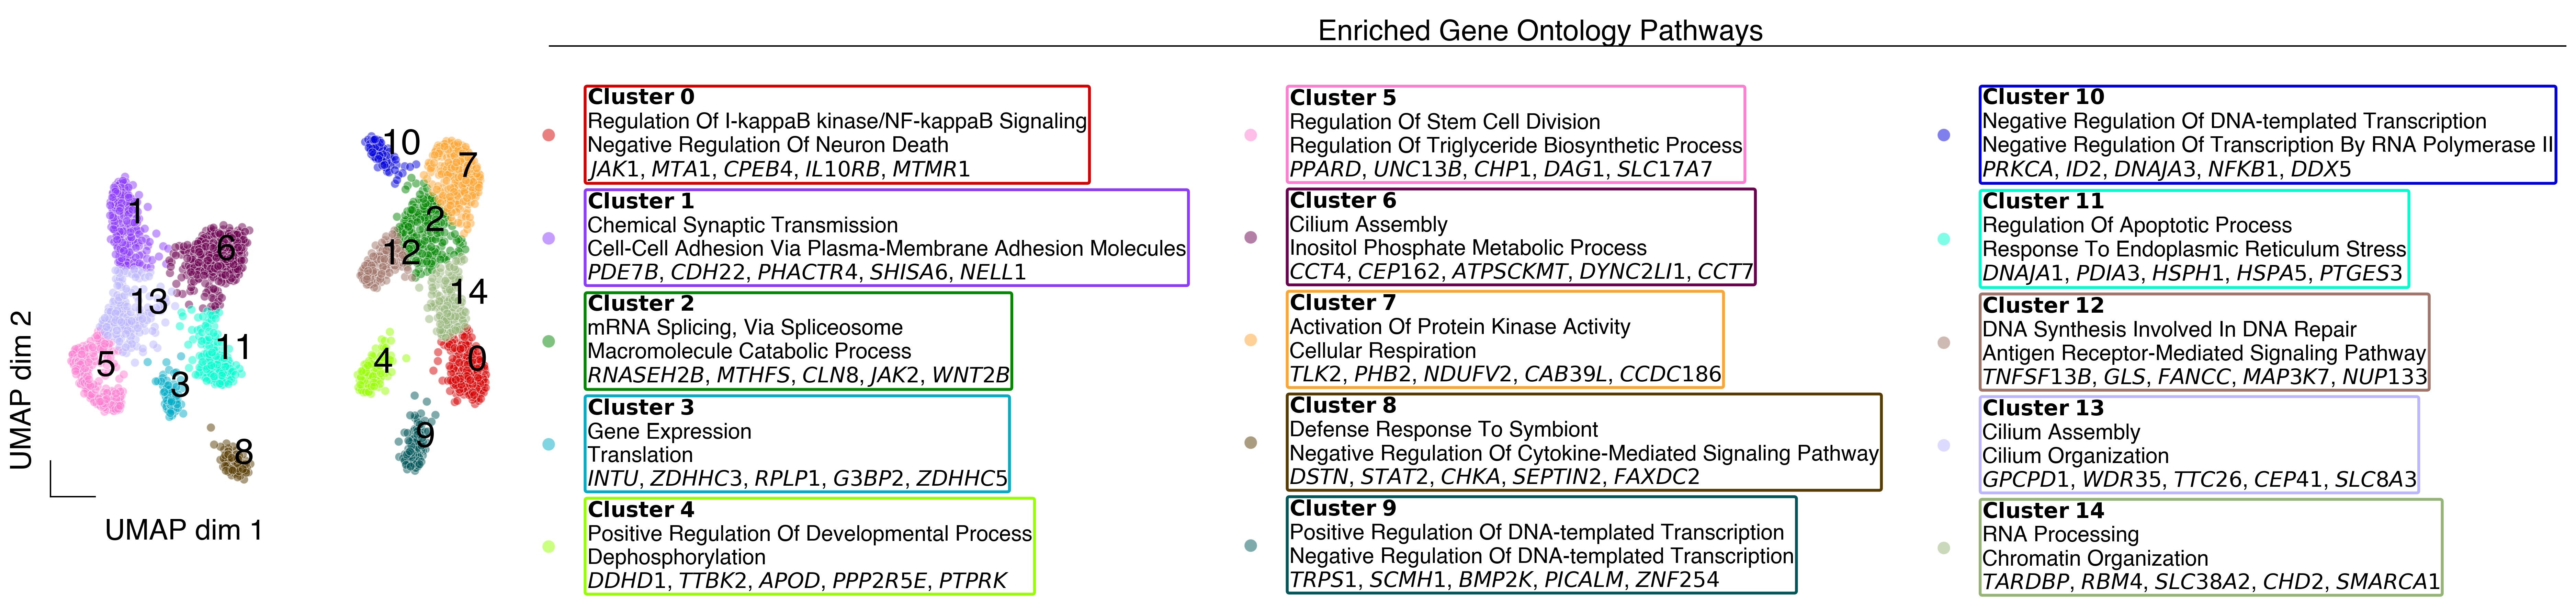
\includegraphics[width=\textwidth]{./main_plots/clusters_umap.png}        
    \end{subfigure}
    \\[-2ex] 
    \begin{subfigure}[t]{\textwidth}
        \caption{}
        
\includegraphics[width=\textwidth]{./main_plots/clusters_bars.png}        
    \end{subfigure}
    \caption{
        \textbf{Single-nuclear RNA-sequencing Atlas of Human Post-mortem Prefrontal Cortex Reveals Cell Type-specific Gene Changes in ABCA7 LoF.}\\
        }
    \label{fig:main_atlas}
\end{figure}
\begin{itemize}
    \item[\textbf{(A)}] ABCA7 gene structure indicating variant locations studied here (average minor allele frequency <1\%). Exons are black rectangles; introns, black lines. Pie chart indicates frequency of ABCA7 PTC-variant carriers in ROSMAP cohort.
    \item[\textbf{(B)}] Overview of human snRNA-seq cohort (created with BioRender.com).
    \item[\textbf{(C)}] Metadata summary of snRNA-seq cohort ($N=32$ individuals).
    \item[\textbf{(D)}] ABCA7 protein abundance in postmortem prefrontal cortex from controls ($N=180$) vs. ABCA7 LoF carriers ($N=5$). Statistical comparison by Wilcoxon rank sum test. Boxes indicate quartiles; whiskers represent data within 1.5× interquartile range.
    \item[\textbf{(E)}] 2D UMAP projection of single-cell gene expression, colored by transcriptionally defined cell type.
    \item[\textbf{(F)}] 2D UMAP projection of ABCA7 LoF gene perturbation scores ($S = -\log_{10}(p)\times\text{sign}(\log_2(\text{FC}))$). Red: $S>1.3$, Blue: $S<-1.3$; point size reflects $|S|$. Up to top 10 genes labeled.
    \item[\textbf{(G)}] 2D UMAP projection colored by gene cluster assignment (Gaussian mixture model; see Methods). Top pathway enrichments per cluster shown (GO BP, hypergeometric enrichment, $p<0.01$).
    \item[\textbf{(H)}] Cell type-specific gene cluster scores ($SC=\text{mean}(S_i)$ for genes $i$ in cluster $c$). * indicates permutation FDR-adjusted $p<0.01$ and $|SC|>0.25$.
\end{itemize}